%TC:envir minted 1 xall 
%TC:envir algorithmic 1 xall

% Include tables in word count
%TC:envir table 0 word
%TC:envir tabular 1 word

% Include footnotes in word count
%TC:macro \footnote [text]
%TC:macro \footnotetext [text]

%TC:group minted 0 0
%TC:macro \mintinline [ignore]
%TC:macro \colb [ignore]
%TC:macro \hyperref [ignore]

\label{sec:1}

The Internet is made up of heterogeneous physical devices running heterogeneous software applications, all trying to interact with each other. This communication is made possible by the unification of data streams in the network layer of the Internet, where information gets routed according to an Internet Protocol (IP). The main focus of the Internet layer is providing maximum reachability. Regardless of the top-level application or bottom-level physical medium being used, every packet gets routed using an IP in the network layer. The shape of the Internet is thus often described as an hourglass, as shown in \cref{fig:intro-hourglass}. 

\begin{figure}[htbp]
  \centering
    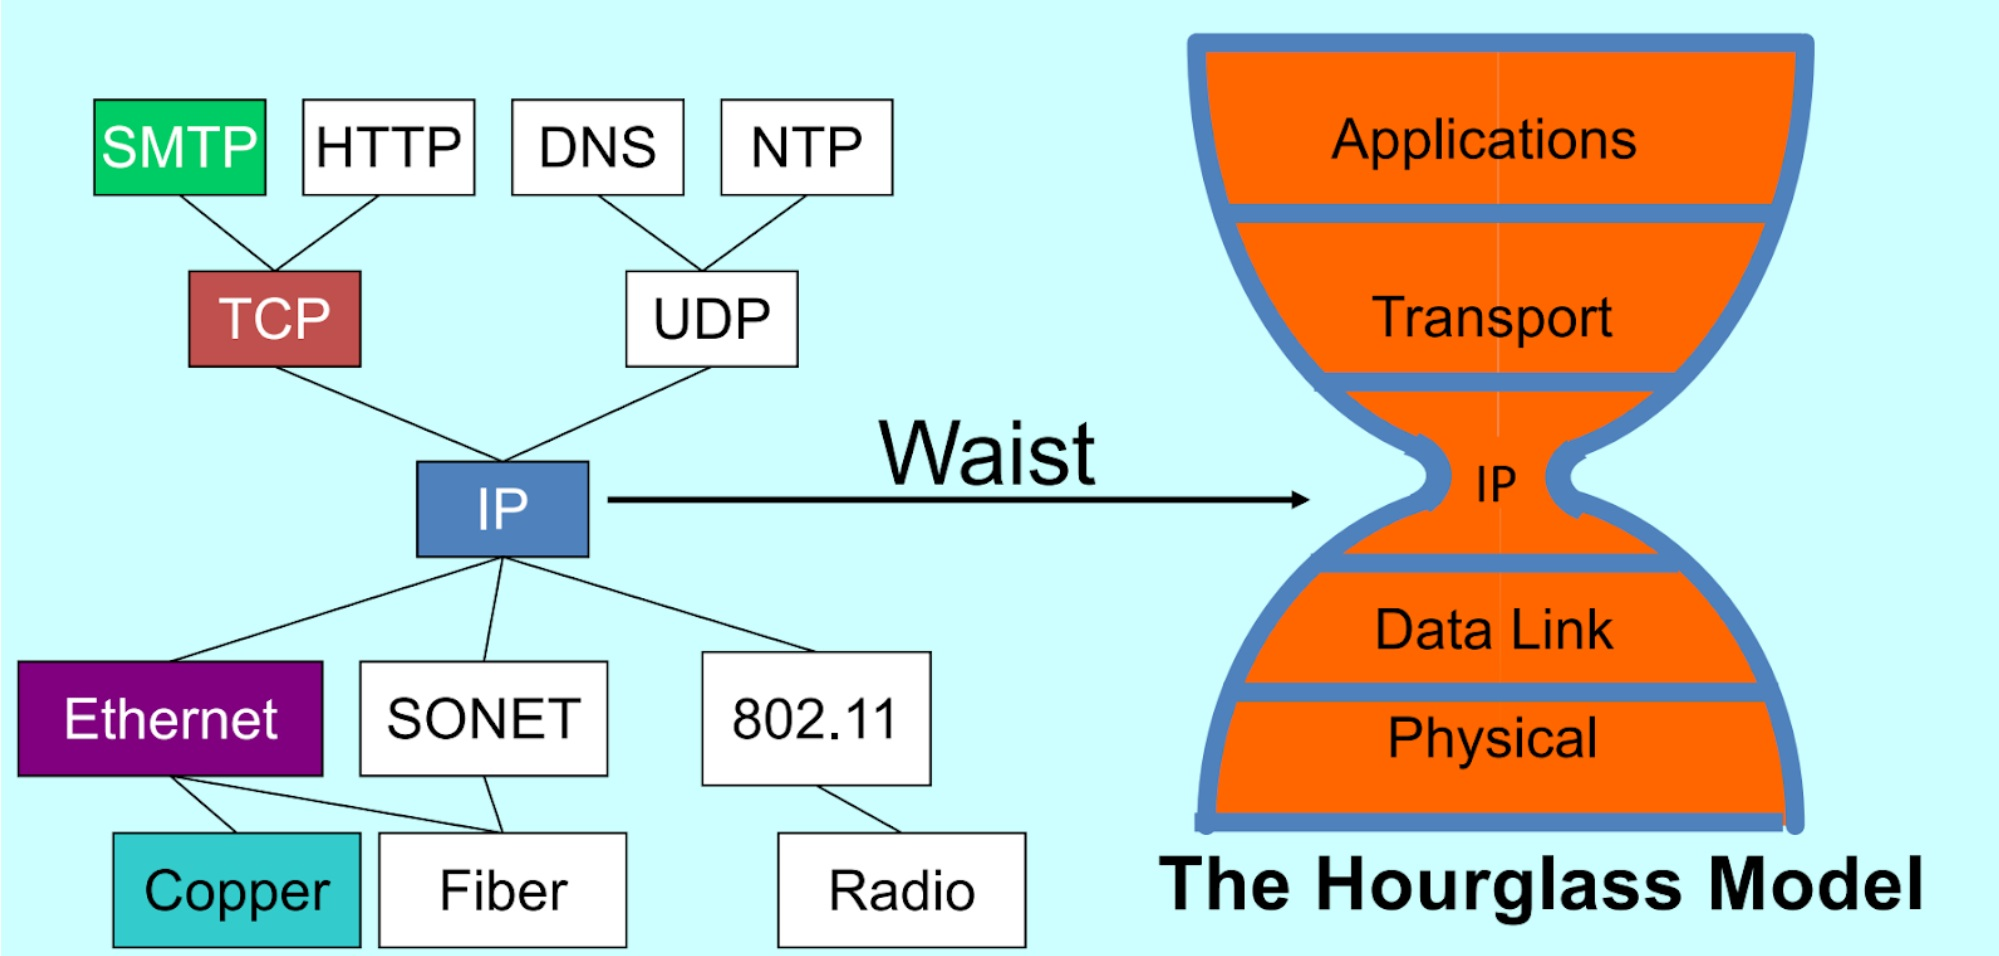
\includegraphics[width=0.65\textwidth]{figures/introduction/hourglass.jpg}
     \caption{The Internet hourglass. Taken from \cite{lectures}.}
     \label{fig:intro-hourglass}
\end{figure}

An IP defines a set of rules that packets need to abide by in order to travel through a network. Upon connecting to the Internet, each node is assigned a unique IP address that allows other devices to locate it anywhere in the world. 

All nodes on the Internet abide by a contract which defines header formats, addressing configurations, datagram structures, and packet handling conventions. Two protocols are currently used in the network layer: IPv4 and IPv6. These protocols coexist in the global Internet, but are mutually incompatible, creating challenges for the migration to one unified IP \cite{lectures}.

IPv4 was released in 1978 and became the globally-accepted Internet standard by the early 1980s \cite{IPv4}. An IPv4 address is 32 bits long and the size of an IPv4 header can vary from 20 to 60 bytes \cite{lectures}. As the Internet started growing exponentially in the late 1980s, IPv4 was anticipated to face an address-space exhaustion problem \cite{IPv6}.  An IPv4 address allows for approximately $2^{32}$ = 4.3 billion unique IP addresses, which was deemed insufficient. This motivated the creation of IPv6, formalised in 1998, which updated the length of an IP address to 128 bits, quadruple the length of an IPv4 address \cite{IPv6}. The address space was hugely increased to $2^{128}$, solving the address-space exhaustion problem \cite{IPv6Paper}. The IPv6 header, which is 40 bytes in length, has been simplified to contain fewer fields than the IPv4 header. A comparison of the two header formats is illustrated in \cref{fig:intro-headers}.

\begin{figure}[htbp]
  \centering
    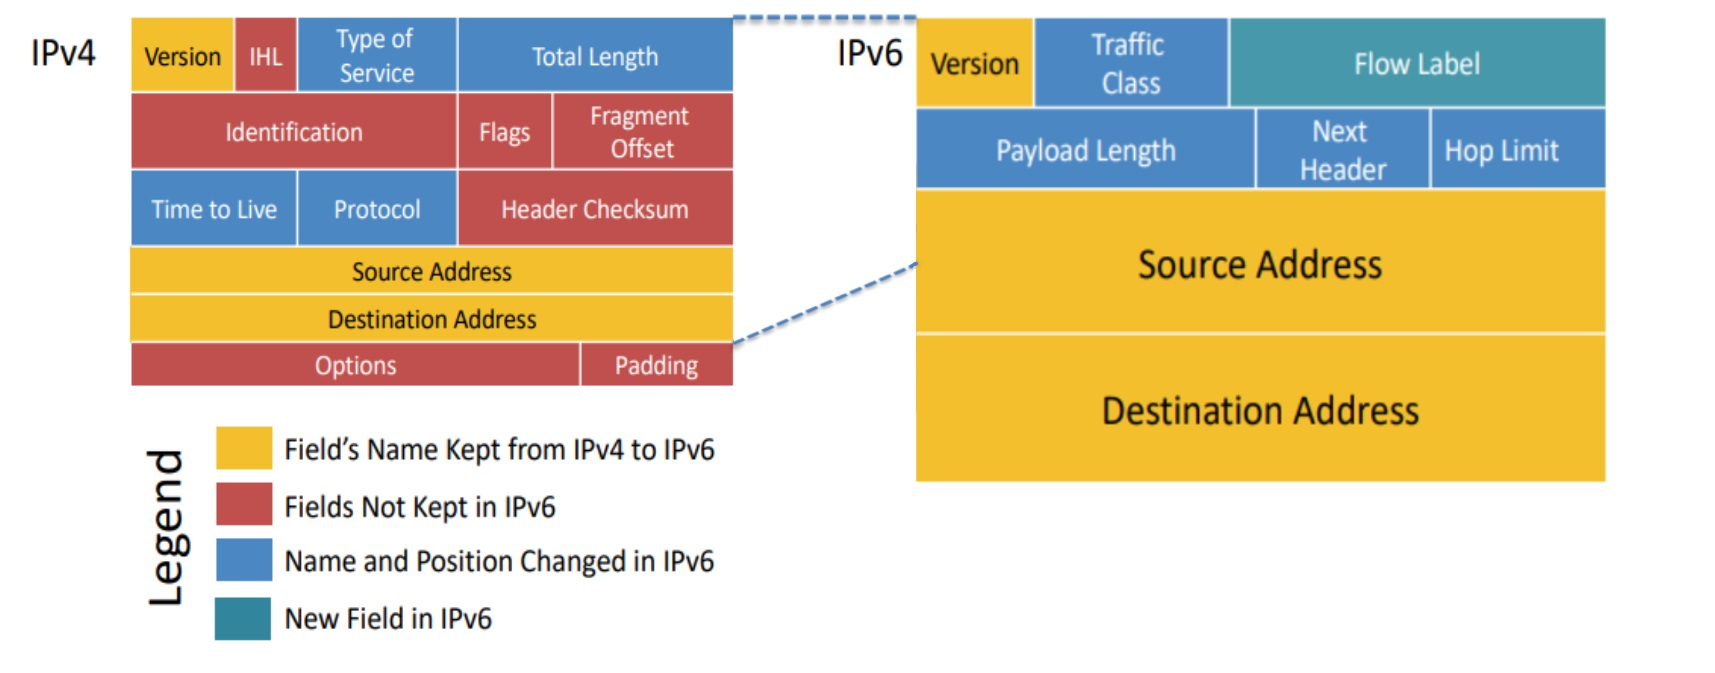
\includegraphics[width=1\textwidth]{figures/introduction/ipv46.jpg}
     \caption{ IPv4 and IPv6 packet header comparison. Adapted from \cite{lectures}.}
     \label{fig:intro-headers}
\end{figure}

Many aspects of the two protocols are incompatible, such as the maximum packet size, fragmentation support, and associated node discovery and diagnostic protocols. IPv4 uses the Address Resolution Protocol (ARP) to discover other nodes on its local network and ICMPv4 for error reporting and signalling. ARP operates below IPv4, while ICMPv4 works on top of IPv4. In IPv6, however, ARP is replaced by the Neighbour Discovery Protocol (NDP), which operates on top of IPv6 and uses ICMPv6 to discover its local network nodes \cite{lectures}.

Due to the various incompatibilities between IPv4 and IPv6, IPv6 adoption rate is still under 50\%, more than 30 years after it was introduced \cite{IPv6Adoption}. Another reason for the low adoption rate is that techniques such as Network Address Translation (NAT) are being used to avoid IPv4's address exhaustion problem. 

A NAT is a device which separates a private network from a public network and allows multiple devices on the private network to access the Internet by using a single public IP address \cite{NAT}. Although this is a widely used workaround, NAT breaks the Internet's end-to-end principle by being a single point of failure (other than the two end hosts) and by requiring information beyond the IP layer (such as port number) to identify nodes in the private network, thus violating security guarantees at the IP level \cite{NATSpecs}. A much more robust solution to the address exhaustion problem would be migrating to IPv6.

Nodes built on IPv4 currently have three options: remain on IPv4, switch to IPv6, or support both. Supporting both IPs can be achieved using various techniques, such as translation, tunneling, or dual IP layering, which are explored in detail in \cref{sec:3.8}. In this dissertation, I refer to a router which implements dual IP layering, i.e. provides separate implementations of both an IPv4 and IPv6 router, as a dual-stack router. Dual-stack nodes bridge the gap between the two IPs and are an essential step in the IPv4-to-IPv6 transition.


\section{Project Summary}
\label{sec:1.1}
The difficulties presented by transitioning from IPv4 to IPv6 motivated my Part II project. I decided to build an IPv6 router on a computer networking platform that does not currently support IPv6. My starting point was the online P4Pi repository, which contains a few example IPv4 functionalities programmed in the domain-specific language (DSL) P4. \cite{P4Pi}. 

In this dissertation I build an IPv6 router prototype, describing in detail the steps I undertake to implement individual functionalities. The core part of my project implements parsing and forwarding in IPv6. Two of the following extensions develop ICMPv6 and NDP functionalities. The final extension examines the nuances involved in extending the router to support both IPv4 and IPv6. This work will highlight the differences between the two IPs and present potential solutions for extending programmable routers to support both.

The evaluation of my project aims to answer the following questions:

\begin{itemize}[topsep=0pt]
\item \textit{Does my router prototype successfully parse, respond to, and forward packets in the manner it was designed to?} At every subtask in Implementation, I state the desired behaviour of the program I am building. I then evaluate the correctness of my programs according to these expectations in \cref{sec:4.1}.

\item \textit{Does my router prototype adhere to Internet Engineering Task Force (IETF) specifications?} In \cref{sec:4.2} I analyze the official technical Internet standards that outline the current best practices for network node behaviour, and I establish that my router prototype adheres to them.

\item \textit{Does the network exhibit significant changes in performance when comparing an IPv4 router, my IPv6 router, and my dual-stack router?} In \cref{sec:4.3} I build a test network and compare the performance of known Internet traffic in both IPs on single- and dual- stack routers to conclude that the difference in efficiency is minimal.

\end{itemize}